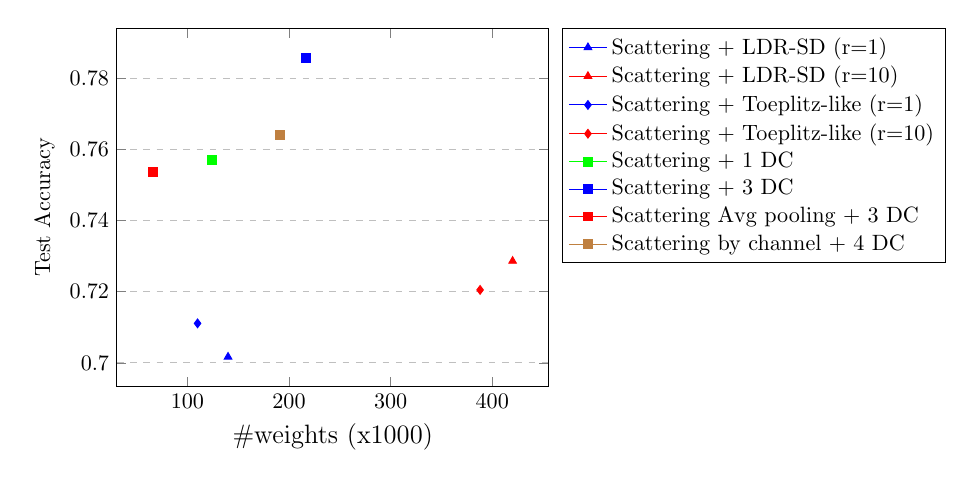
\begin{tikzpicture}[scale=0.8]
\begin{axis}[
    xlabel={\large \#weights (x1000) },
    ylabel={Test Accuracy},
    legend pos=outer north east,
    legend cell align={left},
    ymajorgrids=true,
    grid style=dashed,
    ]
    % \addplot[mark=oplus*,blue] coordinates {(15, 0.6178)}; % Random Conv + Dense
    % \addplot[mark=oplus*,red] coordinates {(90, 0.8438)}; % Conv + Dense
    \addplot[mark=triangle*,blue] coordinates {(140, 0.7017)}; % ldr-sd (rank=1)
    \addplot[mark=triangle*,red] coordinates {(420, 0.7286)}; % ldr-sd (rank=10)
    \addplot[mark=diamond*,blue] coordinates {(110, 0.7111)}; % toeplitz-like (rank=1)
    \addplot[mark=diamond*,red] coordinates {(388, 0.7205)}; % toeplitz-like (rank=10)
    \addplot[mark=square*,green] coordinates {(124, 0.757)}; % Scattering + 1 DC
    \addplot[mark=square*,blue] coordinates {(217, 0.7856)}; % Scattering + 3 DC
    \addplot[mark=square*,red] coordinates {(66, 0.7535)}; % Scattering Avg pooling + 3 DC
    \addplot[mark=square*,brown] coordinates {(191, 0.764)}; % Scattering by channel + 4 DC
    % \addplot[mark=square*,green] coordinates {(131, 0.704)}; % Conv 32 + Max Pooling + 5 DC
    \legend{
        % Random Conv + Dense,
        % Conv + Dense,
        Scattering + LDR-SD (r=1),
        Scattering + LDR-SD (r=10),
        Scattering + Toeplitz-like (r=1),
        Scattering + Toeplitz-like (r=10),
        Scattering + 1 DC,
        Scattering + 3 DC,
        Scattering Avg pooling + 3 DC,
        Scattering by channel + 4 DC,
        % Conv + Max Pooling + DC,
    }
\end{axis}
\end{tikzpicture}

		
